Испытания представляют собой процесс установления соответствия программы и
программной документации заданным требованиям.

\subsection{Проверка требований к документации}
Проверяется наличие всех документов перечисленных в пyнкте 4.1 данного документа и их соответствие ГОСТ.

\subsection{Проверка требований к интерфейсу}
Интерфейс соответствует требованиям, указанным в техническом задании. 

\begin{figure}[h!]
    \centering
    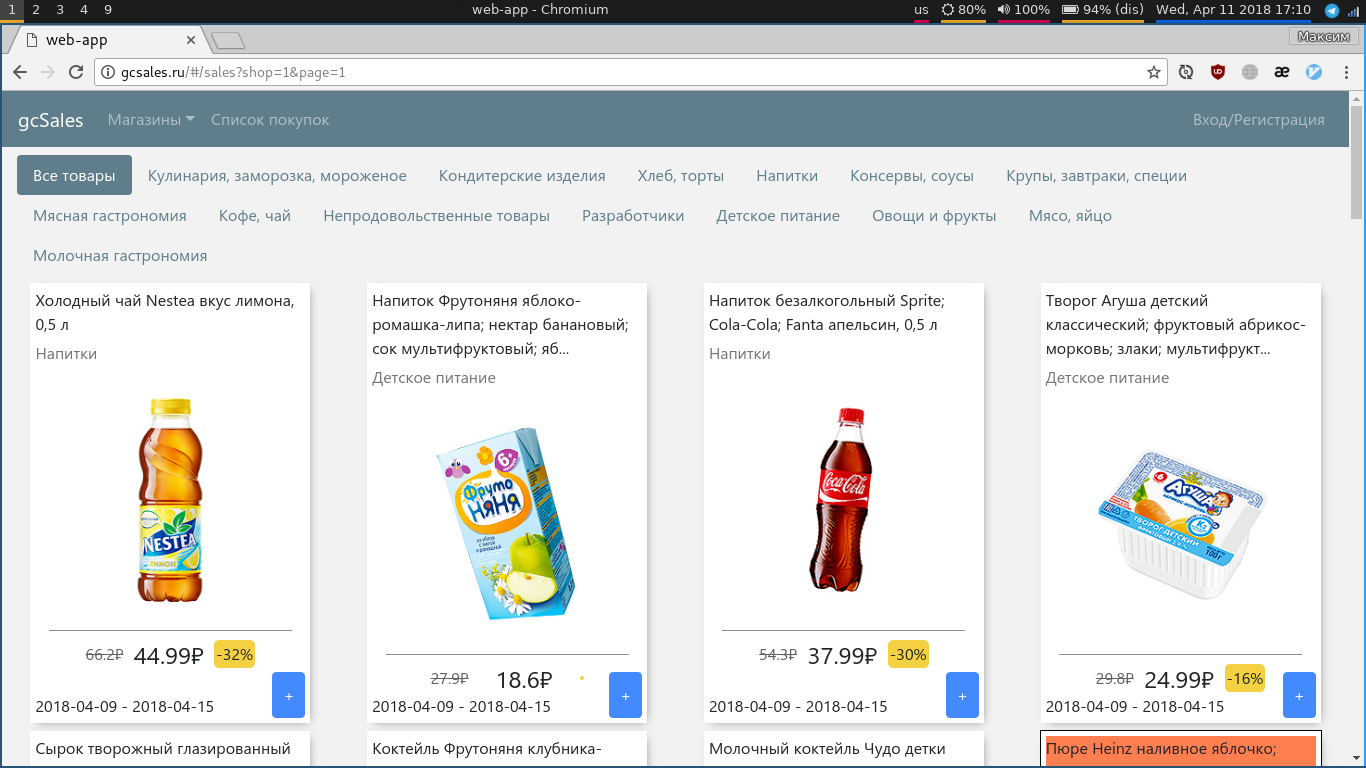
\includegraphics[width=\textwidth]{./screenshots/interface_main.png}
    \caption{Проверка требований к интерфейсу}
    \label{home}
\end{figure}

\newpage
\subsection{Проверка требований к функциональным характеристикам}
\subsubsection{Веб-приложение}
\begin{my_enumerate}
  \item Реализована возможность просмотра списка доступных магазинов с
    акционными товарами
  \item Реализовано представление текущих акций для конкретного магазина:
    \begin{my_enumerate}
      \item В виде общего списка (Рис. 2)
      \item По категориям (Рис. 3)
    \end{my_enumerate}
  \item Реализована возможность регистрации и авторизации пользователей в
    системе для работы со списком покупок (Рис. 4, Рис. 5)
  \item Реализовано создание и удаление списка покупок (Рис. 6, Рис. 7)
  \item Реализована работа со списком покупок:
    \begin{my_enumerate}
      \item Добавление и удаление товаров магазинов
      \item Добавление и удаление пользовательских позиций
      \item Рекомендация товаров магазинов на основе пользовательских позиций
        (Рис. 8)
    \end{my_enumerate}
\end{my_enumerate}

\begin{figure}[h!]
    \centering
    \minipage{0.49\textwidth}
    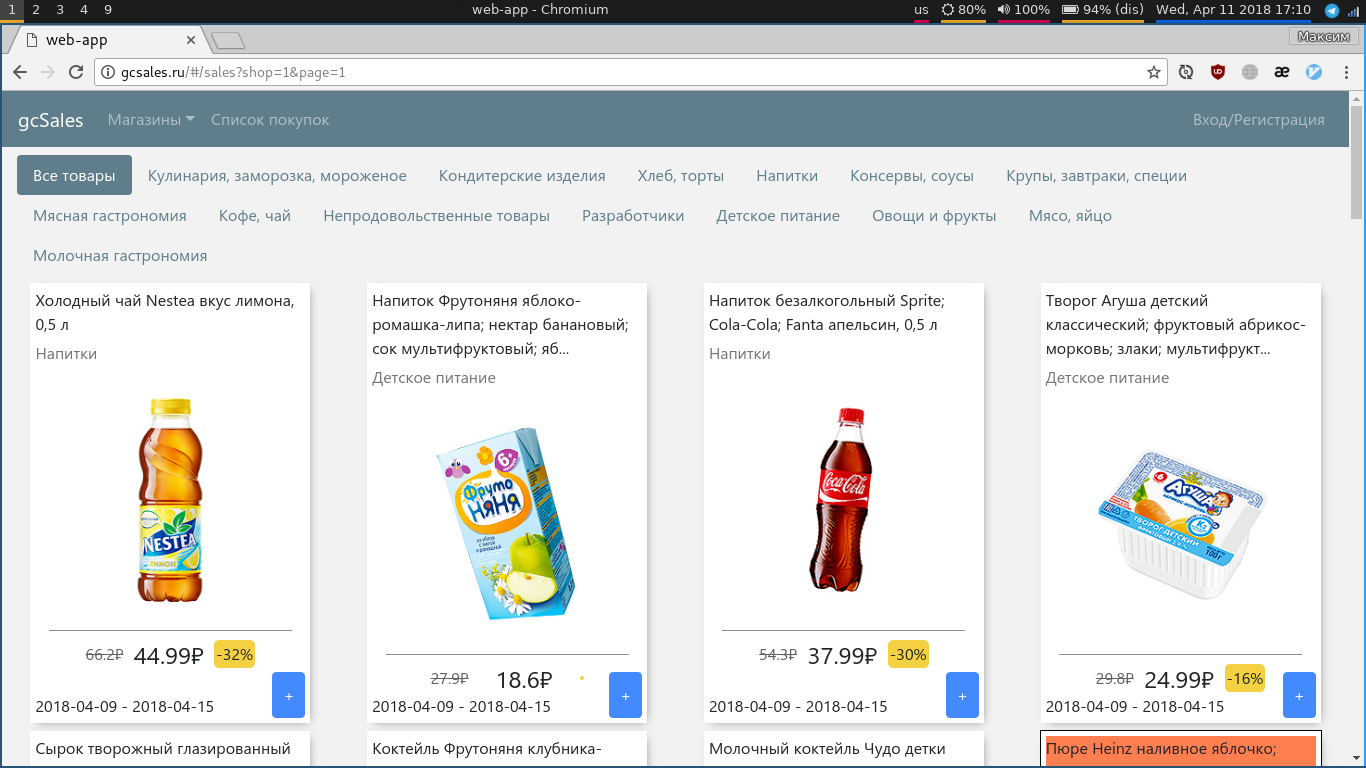
\includegraphics[width=\textwidth]{./screenshots/interface_main.png}
    \caption{Просмотр товаров в виде общего списка}
    \endminipage\hfill
    \minipage{0.49\textwidth}
    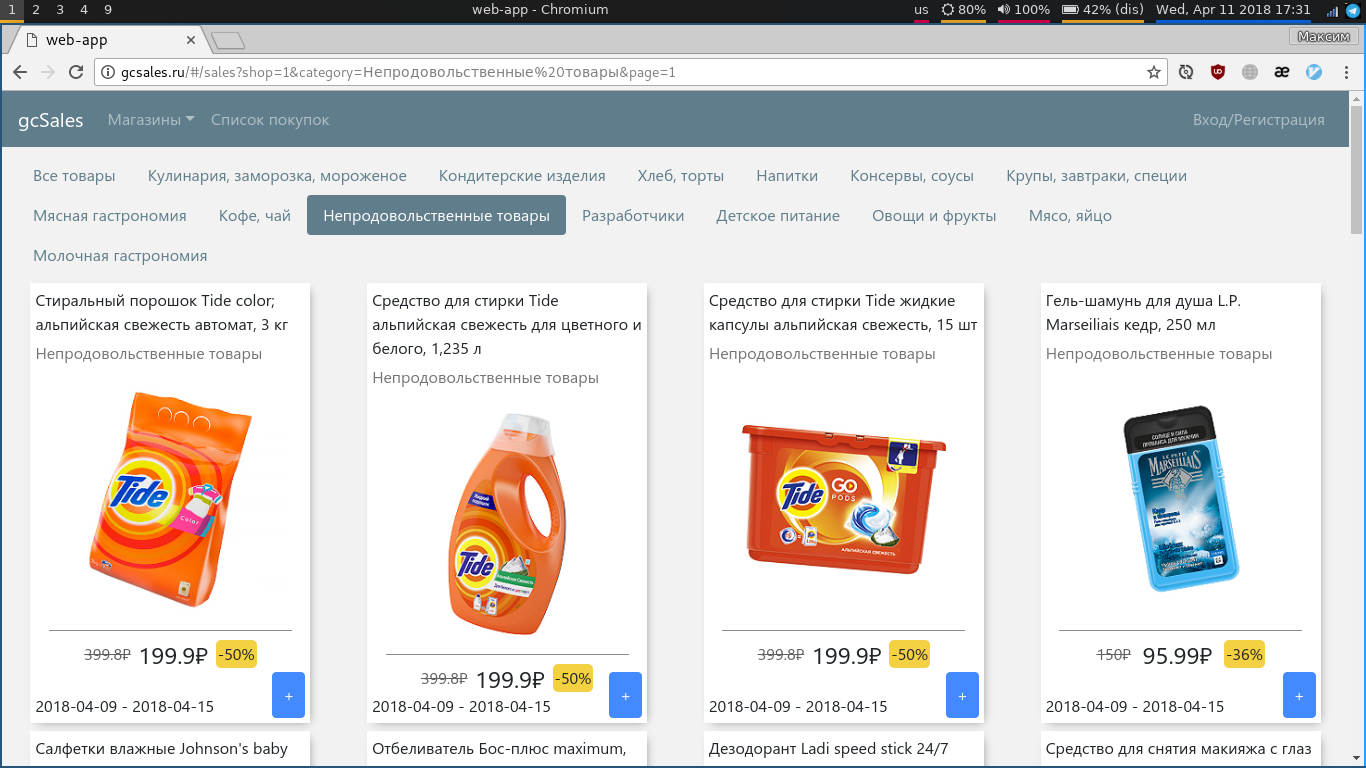
\includegraphics[width=\textwidth]{./screenshots/categories.png}
    \caption{Просмотр товаров категории "Непродовольственные товары"}
    \endminipage
\end{figure}

\begin{figure}[h!]
    \centering
    \minipage{0.49\textwidth}
    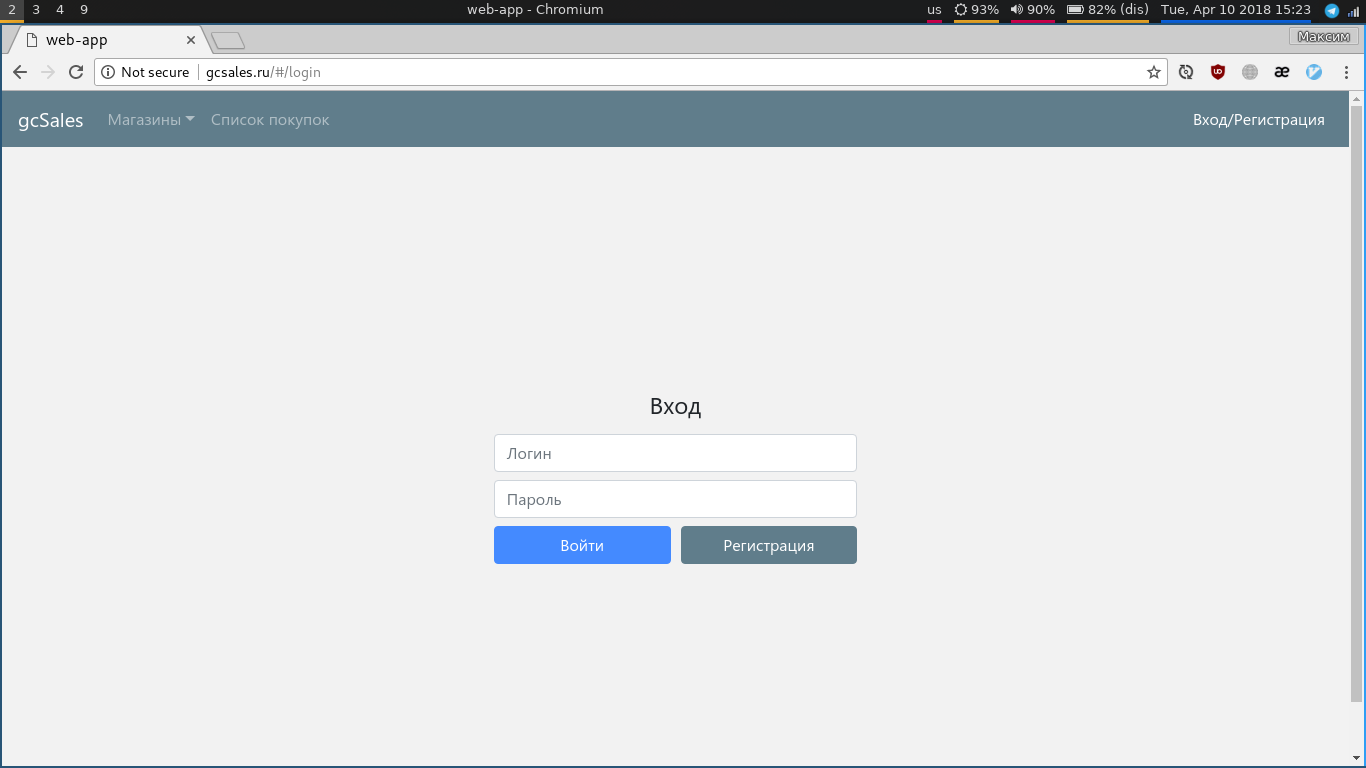
\includegraphics[width=\textwidth]{./screenshots/login.png}
    \caption{Авторизация}
    \endminipage\hfill
    \minipage{0.49\textwidth}
    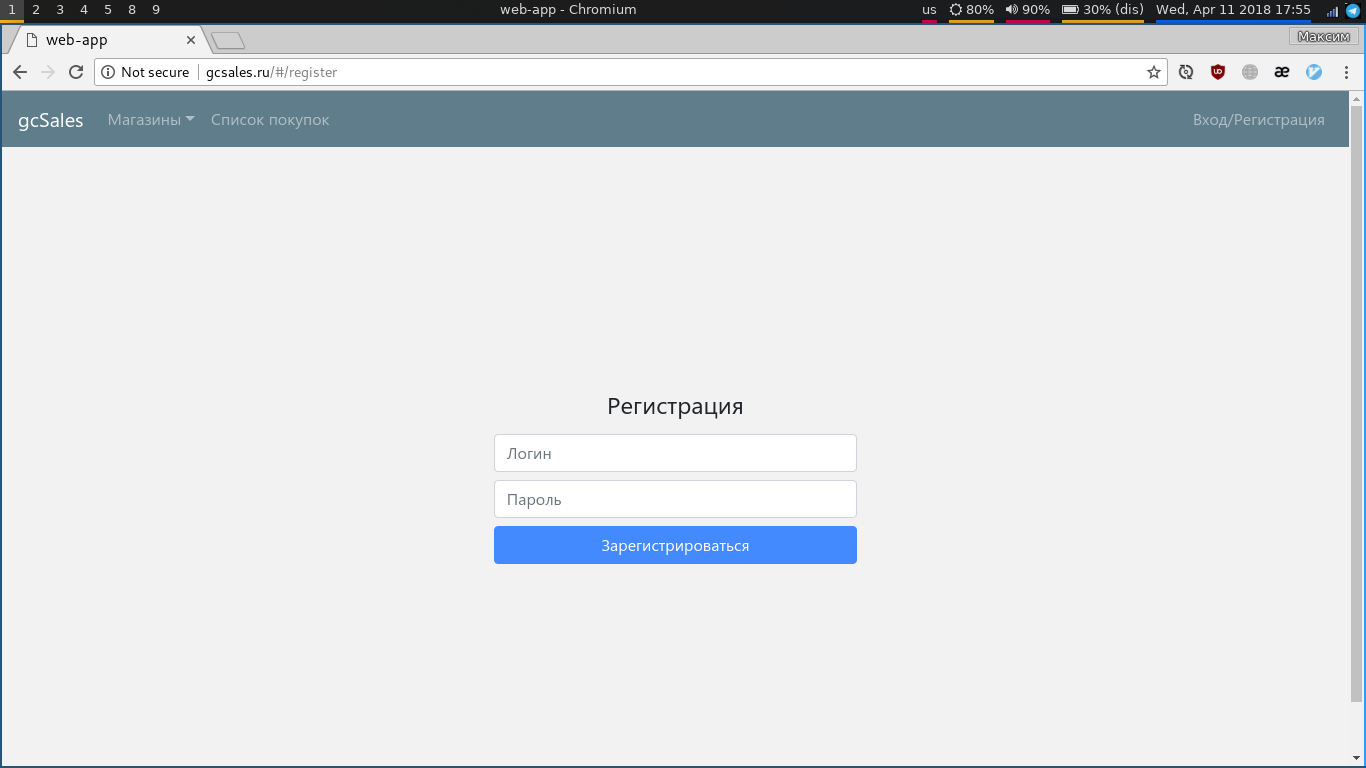
\includegraphics[width=\textwidth]{./screenshots/register.png}
    \caption{Регистрация}
    \endminipage
\end{figure}

\begin{figure}[h!]
    \centering
    \minipage{0.49\textwidth}
    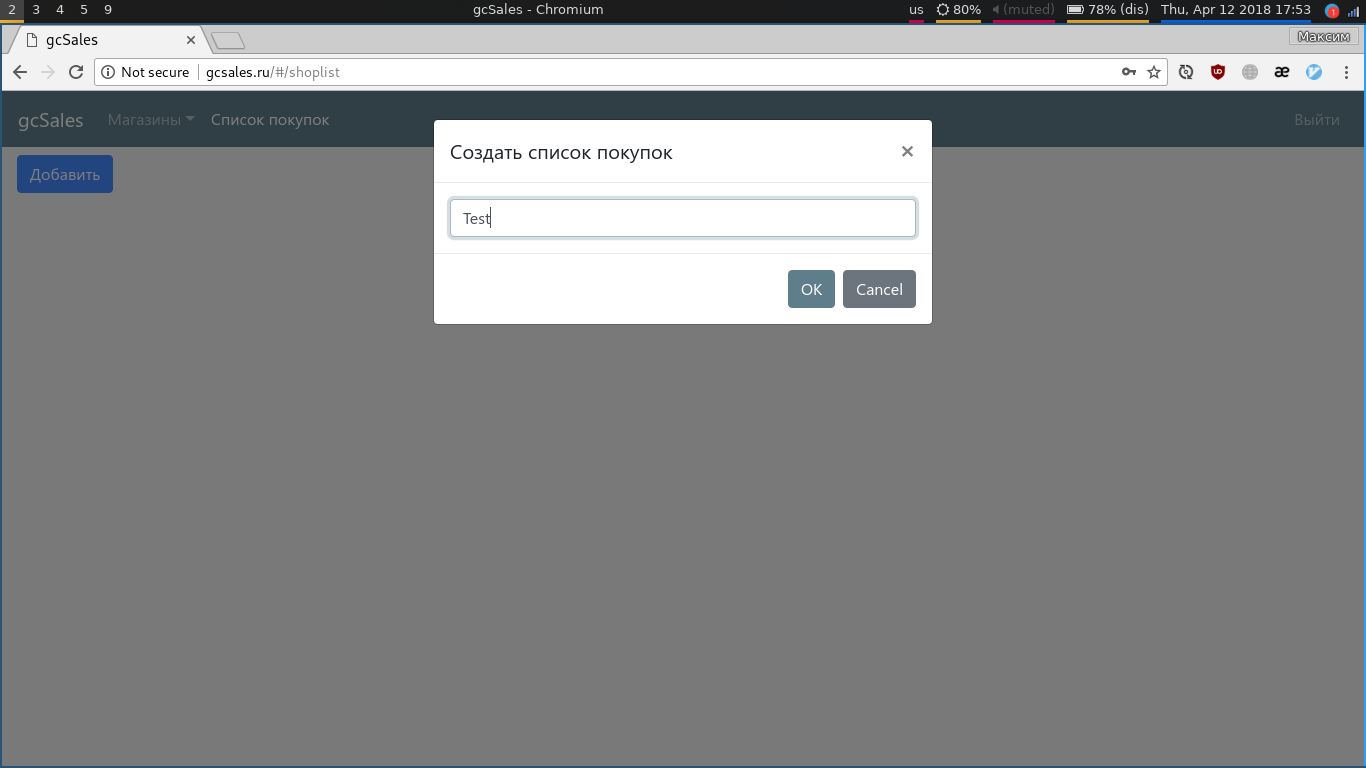
\includegraphics[width=\textwidth]{./screenshots/create_shoplist.png}
    \caption{Создание списка покупок}
    \endminipage\hfill
    \minipage{0.49\textwidth}
    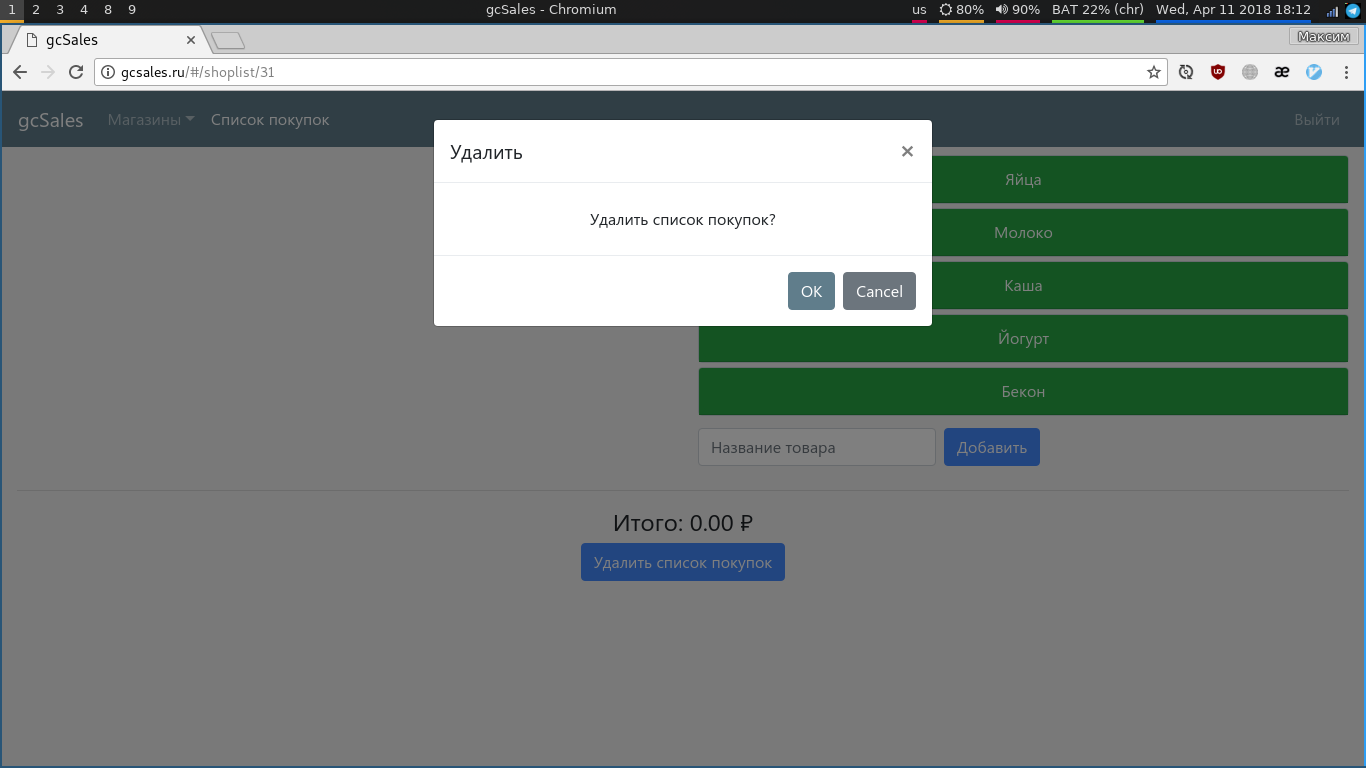
\includegraphics[width=\textwidth]{./screenshots/delete_shoplist.png}
    \caption{Удаление списка покупок}
    \endminipage
\end{figure}

\begin{figure}[h!]
    \centering
    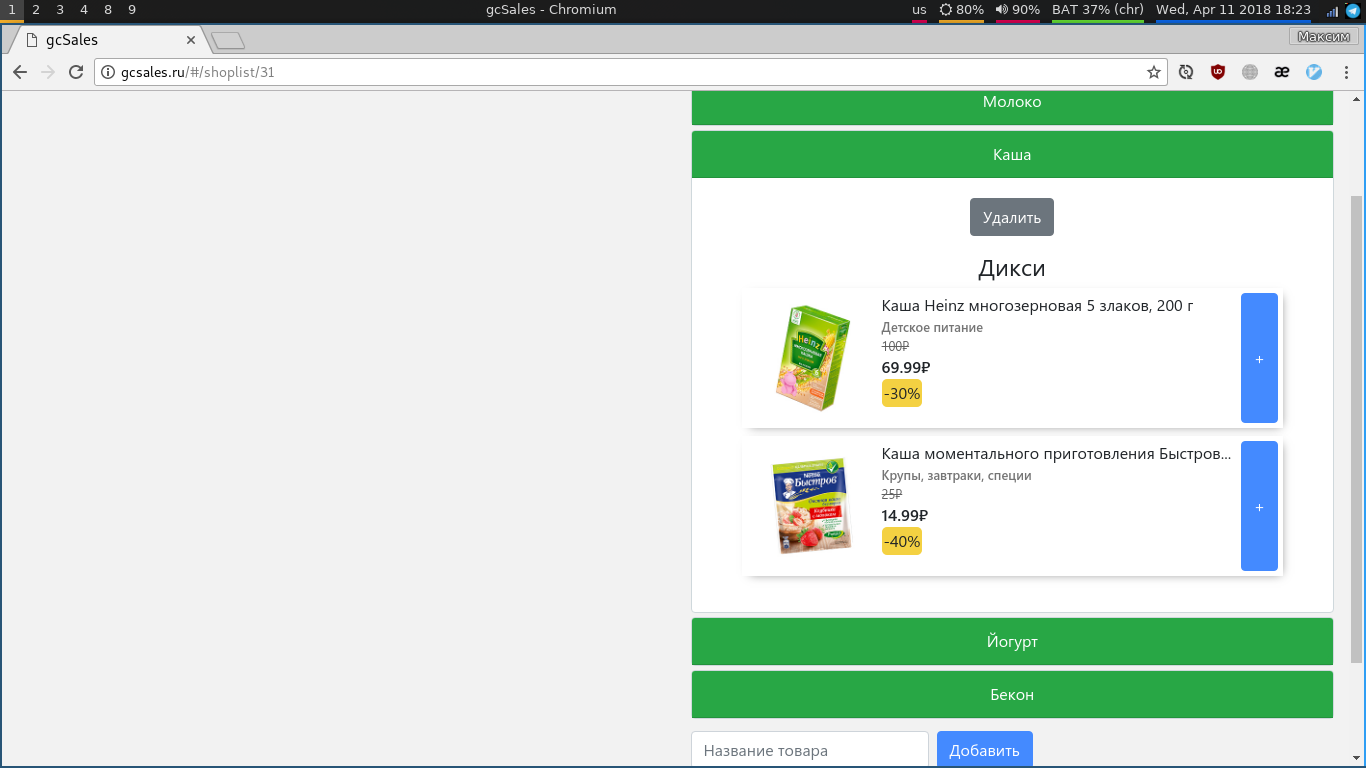
\includegraphics[width=\textwidth]{./screenshots/custom_item.png}
    \caption{Рекомендаци в списке покупок}
\end{figure}

\newpage
\subsubsection{Серверное приложение}
\begin{my_enumerate}
  \item Реализовано REST API (Рис. 9):
    \begin{my_enumerate}
      \item Реализована обработка запросов для работы со списками покупок
        пользователей
      \item Реализована обработка запросов для кроулера
      \item Реализована обработка запросов для получения списка актуальных
        акционных товаров
      \item Реализована обработка запросов для авторизации пользователей
    \end{my_enumerate}
  \item Реализована база данных для хранения (Рис. 10);
    \begin{my_enumerate}
      \item Акционных товаров
      \item Аккаунтов пользователей
      \item Списков покупок пользователей
    \end{my_enumerate}
\end{my_enumerate}

\begin{figure}[h!]
    \centering
    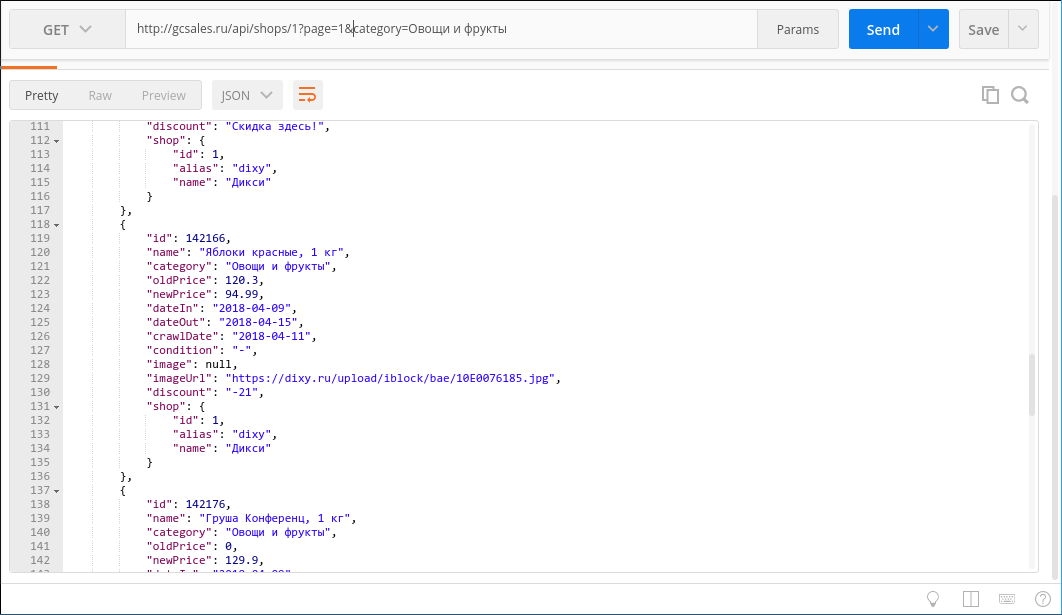
\includegraphics[width=0.7\textwidth]{./screenshots/postman.png}
    \caption{Отправка GET-запроса на сервер и получение ответа}
\end{figure}

\begin{figure}[h!]
    \centering
    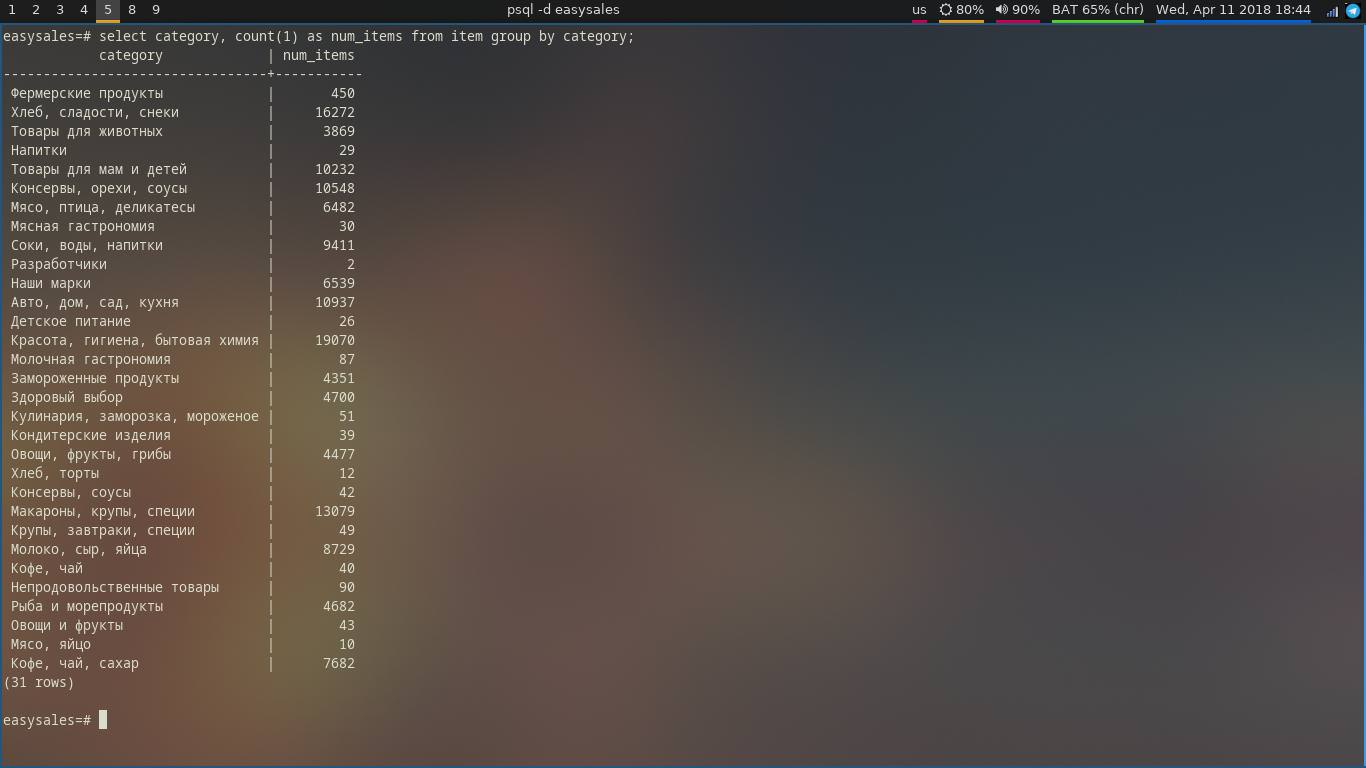
\includegraphics[width=\textwidth]{./screenshots/database.jpg}
    \caption{Работающий запрос к базе данных}
\end{figure}

\newpage
\subsection{Проверка требований к временным характеристикам}
Для проверки требованиям к временным характеристикам было проведено несколько
запросов для получения списка акций.
\begin{figure}[h!]
    \centering
    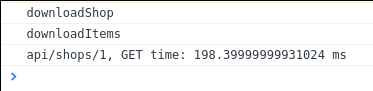
\includegraphics[width=0.5\textwidth]{./screenshots/get1.png}
    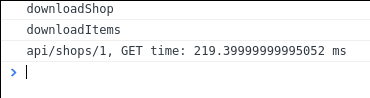
\includegraphics[width=0.5\textwidth]{./screenshots/get2.png}
    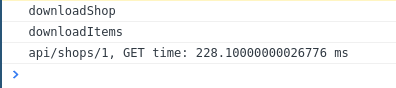
\includegraphics[width=0.5\textwidth]{./screenshots/get3.png}
    \caption{Замер времени отправки запроса}
\end{figure}

Сумма времени на отправку запроса и получения ответа не выходит за допустимые
пределы, описанные в Техническом задании.
